\documentclass[aspectratio=169,11pt]{beamer}

% Slide budget for the whole talk (15 min): at most 12 frames.
%   1 title | 1 XAI | 2 LIME | 3 SHAP | experiments, causation, conclusion | 1 references

\usetheme{Madrid}
\setbeamertemplate{navigation symbols}{}
\setbeamertemplate{footline}[frame number]

\usepackage[utf8]{inputenc}
\usepackage[T1,T5]{fontenc}
\usepackage{lmodern}
\usepackage{amsmath,amssymb,bm}
\usepackage{graphicx}
\usepackage{hyperref}
\usepackage{booktabs}
\usepackage{algorithmic}
\usepackage{tcolorbox}
\tcbuselibrary{skins}
\usepackage{tikz}

\title[LIME and SHAP]{Does an Accurate Prediction Come with a Reliable Explanation?}
\subtitle{A Comparative Study of LIME and SHAP}
\author[Hào, Nam, Phước]{%
  \begin{tabular}{ccc}
    Nguyễn Gia Hào & Phạm Hữu Nam & Nguyễn Hữu Phước \\
    {\small 24125008} & {\small 24125015} & {\small 24125018}
  \end{tabular}}
\institute{APCS -- Faculty of Information Technology\\
VNUHCM - University of Science}
\date{CS420: Intro to AI -- [S04] LIME \& SHAP\\
Instructor: Dr. Nguyễn Ngọc Thảo}

\begin{document}

\begin{frame}
  \titlepage
\end{frame}

% =========================================================
\section{Explainable AI}

\begin{frame}{Explainable AI: key concepts}
  A model flags a tumour as \emph{malignant}; the doctor asks \emph{why}.
  An explanation method answers, but it is itself an algorithm
  with its own assumptions and settings.
  \begin{block}{Guiding question}
    Does a highly accurate prediction necessarily come with a
    reliable explanation?
  \end{block}

  \pause
  {\small
  \begin{itemize}
    \item \textbf{Interpretable vs explainable:} a model a human can follow
      directly (short tree, sparse linear model) vs explanations produced
      for a model that is not.
    \pause
    \item \textbf{Intrinsic vs post-hoc:} interpretable by construction
      vs a separate method explaining an already-trained model.
    \pause
    \item \textbf{Local vs global:} explain one prediction $f(x)$
      vs the model's overall behaviour.
    \pause
    \item \textbf{Model-specific vs model-agnostic:} use the model's
      internals vs only query $f$ as a black box.
  \end{itemize}
  }

  \pause
  \textbf{LIME (2016), SHAP (2017):} post-hoc, local, model-agnostic.
  \emph{Which features pushed this prediction up or down, and by how much?}
\end{frame}

% =========================================================
\section{LIME}

\begin{frame}{LIME: a simple model that is faithful \emph{locally}}
  \begin{columns}[T]
    \begin{column}{0.36\textwidth}
      \centering
      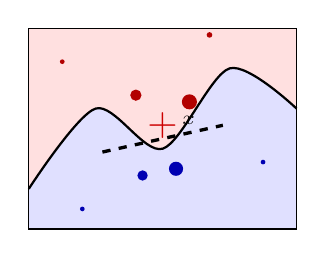
\begin{tikzpicture}[scale=0.85]
        \fill[red!12] (0,3) -- plot[smooth] coordinates
          {(0,0.6) (1,1.8) (2,1.2) (3,2.4) (4,1.8)} -- (4,3) -- cycle;
        \fill[blue!12] (0,0) -- plot[smooth] coordinates
          {(0,0.6) (1,1.8) (2,1.2) (3,2.4) (4,1.8)} -- (4,0) -- cycle;
        \draw[thick] plot[smooth] coordinates
          {(0,0.6) (1,1.8) (2,1.2) (3,2.4) (4,1.8)};
        \draw (0,0) rectangle (4,3);
        % perturbations: radius ~ proximity weight
        \fill[red!70!black]   (2.4,1.9) circle (3.2pt);
        \fill[red!70!black]   (1.6,2.0) circle (2.4pt);
        \fill[red!70!black]   (2.7,2.9) circle (1.2pt);
        \fill[red!70!black]   (0.5,2.5) circle (1.0pt);
        \fill[blue!70!black]  (2.2,0.9) circle (3.0pt);
        \fill[blue!70!black]  (1.7,0.8) circle (2.2pt);
        \fill[blue!70!black]  (3.5,1.0) circle (1.0pt);
        \fill[blue!70!black]  (0.8,0.3) circle (1.0pt);
        % instance and local surrogate
        \draw[very thick, dashed] (1.1,1.15) -- (2.9,1.55);
        \node[red!80!black, font=\Large\bfseries] at (2.0,1.55) {$+$};
        \node[font=\scriptsize, anchor=west] at (2.15,1.62) {$x$};
      \end{tikzpicture}

      {\scriptsize Shading: decision of $f$.
      Dot size: weight $\pi_x$.
      Dashed: local linear $g$.}
    \end{column}
    \begin{column}{0.62\textwidth}
      {\small
      Explain $f(x)$ by a simple $g$ that only has to match $f$
      on \emph{variations of $x$} (inputs similar to $x$).

      \pause
      \vspace{0.3em}
      \textbf{Interpretable representation}
      $x'=(1,\dots,1)\in\{0,1\}^{d'}$:
      bit $j$ $=$ ``unit $j$ present''
      (a word, a super-pixel, a value range).
      $g$ sees $x'$ and should give $g(x')\approx f(x)$.

      \pause
      \vspace{0.3em}
      \textbf{Variations:} switch off random bits,
      map back with $h_x$; $g$ sees $z'$, $f$ sees $z$:\\[0.2em]
      \hspace*{1em}$x'=(1,1,1,1)\xrightarrow{h_x}$ ``the food was great''\\
      \hspace*{1em}$z'=(1,0,1,1)\xrightarrow{h_x}$ ``the was great''
      }
    \end{column}
  \end{columns}

  \pause
  \vspace{0.2em}
  Want $g(z')\approx f(z)$, weighted by proximity
  $\pi_x(z)=\exp\bigl(-D(x,z)^2/\sigma^2\bigr)$:
  \[
    \xi(x)=\arg\min_{g\in G}\;
    \underbrace{\sum_{(z,z')}\pi_x(z)\bigl(f(z)-g(z')\bigr)^2}_{\mathcal{L}(f,g,\pi_x):\ \text{faithful}}
    +\underbrace{\Omega(g)}_{\text{readable}} .
  \]
  {\small
  \pause
  \textbf{In LIME:} sparse linear $g(z')=w_g\cdot z'$;
  \ $\Omega(g)=\infty$ if more than $K$ weights are non-zero, else $0$.
  }
\end{frame}

\begin{frame}{LIME: output and limitations}
  \vspace{0.3em}
  {\small
  \textbf{In practice:} sample $N$ variations ($N$ calls to $f$),
  weight them by $\pi_x$, fit $g$ with ``K-LASSO''
  (Lasso picks $K$ units, then weighted least squares on them).
  }

  \vspace{0.4em}
  \begin{columns}[T]
    \begin{column}{0.42\textwidth}
      \pause
      {\small
      \textbf{Output:} $K$ signed weights.
      \textcolor{red!70!black}{$w_j>0$} supports the class,
      \textcolor{blue!70!black}{$w_j<0$} opposes it.
      }

      \vspace{0.3em}
      \centering
      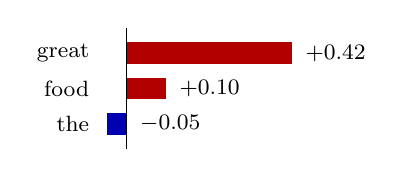
\begin{tikzpicture}[x=5cm, y=0.45cm, font=\footnotesize]
        \fill[red!70!black]  (0,2.7) rectangle (0.42,3.3);
        \fill[red!70!black]  (0,1.7) rectangle (0.10,2.3);
        \fill[blue!70!black] (0,0.7) rectangle (-0.05,1.3);
        \draw (0,0.3) -- (0,3.7);
        \node[anchor=east] at (-0.07,3) {great};
        \node[anchor=east] at (-0.07,2) {food};
        \node[anchor=east] at (-0.07,1) {the};
        \node[anchor=west] at (0.43,3) {$+0.42$};
        \node[anchor=west] at (0.11,2) {$+0.10$};
        \node[anchor=west] at (0.01,1) {$-0.05$};
      \end{tikzpicture}

      {\scriptsize ``the food was great'', class \emph{positive},
      $K=3$ (illustrative numbers).}
    \end{column}
    \begin{column}{0.54\textwidth}
      \pause
      \textbf{Limitations}
      {\small
      \begin{itemize}
        \item No local accuracy: $g(x')$ need not equal $f(x)$.
        \pause
        \item Depends on the random variations, $N$, $\sigma$
          and the representation.
        \pause
        \item Variations may be unrealistic;
          kernel and penalty are heuristic.
      \end{itemize}
      }
    \end{column}
  \end{columns}

  \pause
  \begin{block}{Next: SHAP}
    Which kernel and penalty make the explanation \emph{unique},
    with guaranteed properties?
  \end{block}
\end{frame}

% =========================================================
\section{SHAP}

\begin{frame}{SHAP: additive feature attribution}
  \begin{columns}[T]
    \begin{column}{0.55\textwidth}
      {\small
      Same setting as LIME: a linear $g$ on $z'\in\{0,1\}^M$,
      \[
        g(z')=\phi_0+\sum_{j=1}^{M}\phi_j z'_j ,
      \]
      $z'_j=1$: feature $j$ \emph{known} (keeps $x_j$),
      $z'_j=0$: \emph{missing}.

      \pause
      \vspace{0.3em}
      \textbf{Missing} $=$ averaged out over a background
      (reference rows $b$):
      \[
        f_x(S)=\mathbb{E}[f(z)\mid z_S=x_S]
        \approx\mathbb{E}_b\bigl[f(x_S,b_{\bar S})\bigr].
      \]
      \textbf{Base value} $\phi_0=f_x(\varnothing)$:
      the average prediction.

      \pause
      \vspace{0.3em}
      \textbf{Sign:} $\phi_j>0$ pushes the output above $\phi_0$,
      $\phi_j<0$ below.
      }
    \end{column}
    \begin{column}{0.43\textwidth}
      \pause
      \centering
      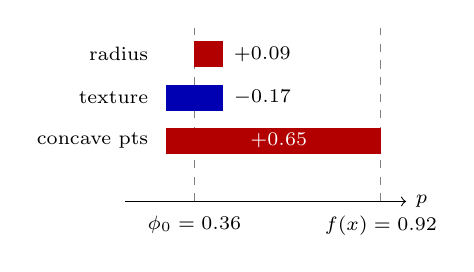
\begin{tikzpicture}[x=4.2cm, y=0.55cm, font=\scriptsize]
        \draw[dashed, gray] (0.360,0.6) -- (0.360,4.6);
        \draw[dashed, gray] (0.924,0.6) -- (0.924,4.6);
        \fill[red!70!black]  (0.360,3.7) rectangle (0.446,4.3);
        \fill[blue!70!black] (0.446,2.7) rectangle (0.275,3.3);
        \fill[red!70!black]  (0.275,1.7) rectangle (0.924,2.3);
        \node[anchor=east] at (0.25,4) {radius};
        \node[anchor=east] at (0.25,3) {texture};
        \node[anchor=east] at (0.25,2) {concave pts};
        \node[anchor=west] at (0.45,4) {$+0.09$};
        \node[anchor=west] at (0.45,3) {$-0.17$};
        \node[anchor=west] at (0.50,2) {\color{white}$+0.65$};
        \draw[->] (0.15,0.6) -- (1.0,0.6) node[right] {$p$};
        \node[anchor=north] at (0.360,0.5) {$\phi_0=0.36$};
        \node[anchor=north] at (0.924,0.5) {$f(x)=0.92$};
      \end{tikzpicture}

      {\scriptsize \emph{Ours}: 3-feature logistic regression on
      Breast Cancer; output $=$ probability of malignant.
      $0.36+0.09-0.17+0.65=0.92$.}
    \end{column}
  \end{columns}
\end{frame}

\begin{frame}{Shapley values: the unique split with three properties}
  \vspace{0.2em}
  {\small
  \begin{itemize}
    \item \textbf{Local accuracy:} $f(x)=\phi_0+\sum_j\phi_j$
      \quad (LIME does not guarantee this).
    \pause
    \item \textbf{Missingness:} a unit absent from $x$ ($x'_j=0$)
      gets $\phi_j=0$.
    \pause
    \item \textbf{Consistency:} if $j$'s marginal contributions never
      decrease, $\phi_j$ does not decrease.
  \end{itemize}
  }

  \pause
  \begin{block}{Theorem 1: only the Shapley values satisfy all three}
    \[
      \phi_j=\sum_{S\subseteq\{1,\dots,M\}\setminus\{j\}}
      \frac{|S|!\,(M-|S|-1)!}{M!}
      \bigl[f_x(S\cup\{j\})-f_x(S)\bigr]
    \]
  \end{block}

  \pause
  {\small
  Reveal features in a random order: $\phi_j$ $=$ average jump of the
  output when $j$ is revealed.\\[0.2em]
  \emph{Example:} score $0$ (no symptom), $5$ (fever or cough alone),
  $2$ (both):
  $\phi_{\text{fever}}=\tfrac12[(5-0)+(2-5)]=1=\phi_{\text{cough}}$,
  \ $0+1+1=2=f(x)$.
  }
\end{frame}

\begin{frame}{Computing SHAP values}
  \textbf{Kernel SHAP} (Theorem 2): LIME's objective gives exactly
  the Shapley values with
  {\small
  \[
    \Omega(g)=0,
    \qquad
    \pi_x(z')=\frac{M-1}{\binom{M}{|z'|}\,|z'|\,(M-|z'|)},
    \qquad
    \text{constraints } \phi_0=f_x(\varnothing),\ \textstyle\sum_j\phi_j=f(x)-\phi_0 .
  \]
  }

  \pause
  \vspace{-0.3em}
  \begin{center}
    \footnotesize
    \begin{tabular}{lll}
      \toprule
      & LIME & Kernel SHAP \\
      \midrule
      Weight of a variation & proximity, width $\sigma$ by hand
        & coalition size only, no width \\
      Complexity $\Omega$ & at most $K$ weights & none \\
      Constraints & none & local accuracy \\
      Result & heuristic weights & Shapley values (enough samples) \\
      \bottomrule
    \end{tabular}
  \end{center}

  \pause
  {\small
  \textbf{Model-specific:}
  Linear SHAP $\phi_j=w_j\,(x_j-\mathbb{E}[x_j])$ in closed form;
  Tree SHAP exact for tree ensembles.
  }

  \pause
  \vspace{0.3em}
  {\small
  \textbf{Caveats:} sampling noise for non-linear $f$; $\phi_0$ and all
  $\phi_j$ depend on the background; independence creates unrealistic
  inputs for correlated features.
  }
\end{frame}

% =========================================================
\begin{frame}{References}
  \begin{enumerate}
    \item M.~T.~Ribeiro, S.~Singh, C.~Guestrin.
      ``Why Should I Trust You?'': Explaining the Predictions of Any
      Classifier. \emph{KDD}, 2016.

    \item S.~M.~Lundberg, S.-I.~Lee.
      A Unified Approach to Interpreting Model Predictions.
      \emph{NeurIPS}, 2017.

    \item S.~M.~Lundberg et al.
      From local explanations to global understanding with explainable
      AI for trees. \emph{Nature Machine Intelligence}, 2:56--67, 2020.

    \item Explainable artificial intelligence: A survey of needs,
      techniques, applications, and future direction.
      \emph{Neurocomputing}, 599:128111, 2024.
  \end{enumerate}
\end{frame}

\end{document}
